% This is "Model.tex"
% A content sub-file for Trustfull Action Suggestion Thesis Extended Abstract

\section{Trust Model}
\label{sec:TrustModel}
We sought out to develop a trust model definition that would be easily implementable, but generic enough to be able to adapt to various testing scenarios. To do this we took inspiration from the work by Sabater et al.\cite{Sabater2006} described in Section \ref{subsubsec:Related work:Trust Models:Repage} by taking a similar approach to architecture where a central memory component holds the model's current state, getting updated by perceptions received from the environment. But while Repage describes a third module that suggests actions to resolve belief conflicts in the model, we instead defined such module to assume the point of view of one of the agents in the scenario and, if participating in a social interaction, it suggests actions to improve the trust relationship with a trustor. In fact, most of the design of the model was made with the intent that it would be used by one of the agent's in the scenario, and the model created would be his own trust model of the world environment. And so, the model can be described by 3 main components:
\begin{itemize}
    \item \textbf{Memory}, which defines and stores the main model structure;
    \item \textbf{Perceptions}, a series of environment perceptions mapped to changes in the Memory;
    \item \textbf{Action Suggestion}, a module that outputs different actions depending on current perceptions and the state of the model.
\end{itemize}

\subsection{Memory}
One of the main concerns while designing the model was how trust would be calculated, as we wanted to use Castlefranchi and Falcone's conceptualization of trust \cite{Castelfranchi2010} as a basis for trust definition, focusing specially on it being dependent on the task entrusted, and the transferability of trust between different tasks. But starting from the five-part definition of trust, as seen in Equation \ref{eq:TrustRelation}, we decided that inserting context (\textbf{C}) and the trustor's goal (\bm{$g_x$}) into the model would bring in too much complexity for the scope of this thesis, as it would require for a world state model to be kept, as well as some way to predict the trustor's goal. So we simplified, defining trust through a simpler three-part relation, involving just the trustor (\textbf{X}), the trustee (\textbf{Y}) and the task ($\bm{\tau}$), represented in Equation \ref{eq:TrustCalc}.
\begin{equation}
TRUST(X\ Y\ \tau)
\label{eq:TrustCalc}
\end{equation}

So we designed the structure with the concepts and relations represented in Figure \ref{fig:MemoryArchitecture}, and we can describe them as follows:

\begin{itemize}
    \item \textbf{Agent}: a simple representation of the known entities in the scenario world space, serving mostly as an identifier;
    \item \textbf{Trustee}: each agent contains a collection of other agents he has information about,  either by reputation, or by interaction, which we represent as their Trustees;
    \item \textbf{Trust Feature}: a piece of information a trustor has on a trustee is represented in a Trust Feature, which contains the Belief Sources of said information. The Feature Model defines and uniquely identifies what feature is represented.
    \item \textbf{Feature Model}: the possible set of trust features from which a trustee can be assigned is defined in a collection of Feature Models where each one represents a possible piece of trust related information relevant to the model scenario (e.g. The trustee's ability to cook, or the willingness to drive);
    \item \textbf{Category}: a Feature Model must belong to a Category, making it easier to present the different type of Trust Features;
    \item \textbf{Belief Source}: this represents a source of information on the corresponding feature, belonging to one of the 3 sub-classes depending on the origin of the information, Reputation for when reported from other agents (whether directly (e.g. talking) or indirectly (e.g. report on newspaper)), Bias for pre-existing beliefs on the feature, and Direct Contact for direct observations of the trustee, 3 values are provided to determine the associated feature's belief value: 
        \begin{itemize}
            \item Belief Value, a number between 0.0 and 1.0 describing the trustor evaluation;
            \item Certainty describes how well the trustee was evaluated, in Reputation for instance, this might represent how well we trust in the reporter, and in Direct Contact how well the trustor observed the trustee performing said feature;
            \item Time is just a record of when was this belief source recorded, as older records might have a lower impact in the overall belief value score, compared to newer records.
        \end{itemize} 
    \item \textbf{Task}: a representation of the possible delegation tasks in the scenario, containing the Feature Models associated with the performance of this task (e.g. The ability to serve drinks if the task is bartending). A weight is given to each Feature corresponding to its importance in the task. The various weights are normalized so that their sum is 1.0.
\end{itemize} 

\begin{figure}[hbt]
    \centering
    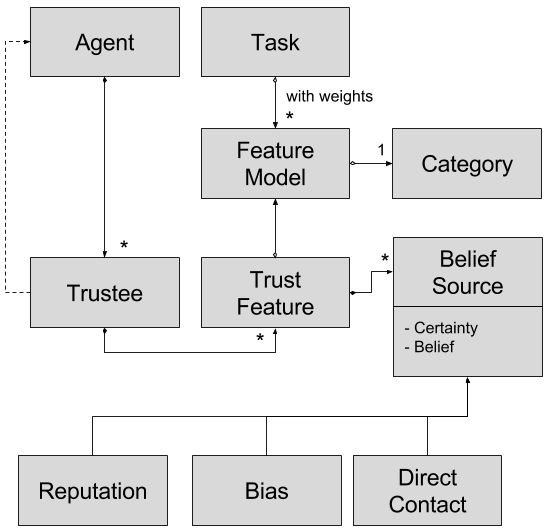
\includegraphics[width=200px]{TrustMemoryDiagram.png}
    \caption{Memory Architecture (represented in UML)}
    \label{fig:MemoryArchitecture}
\end{figure}


\subsubsection{Trust Calculation}
Taking a Trustor $X$, a Trustee $Y$ and a delegated task $\tau$, Trust can then be calculated by taking the Trustee's Trust Features $F_y$, the Task's Feature Models $F_\tau$ and checking which they have in common, which we can represent as $F_{y\cap\tau}$~. Remember that Trust Features are uniquely identified by a Feature Model. So after getting $F_{y\cap\tau}$ we can apply a linear function to each of the features in $F_{y\cap\tau}$, where for each element $F_i$ we multiply the trustee's feature's belief value $B(F_i)$ with the weight of the feature for the task $W(F_i)$, as represented in Equation \ref{eq:TrustCalculation}.
\begin{equation}
    Trust_{X,Y,\tau}=\sum_{i=0}^{n}W(F_i) B(F_i)
    \label{eq:TrustCalculation}
\end{equation}

The belief value of the feature itself, $B(F_i)$, is also calculated through a sum of parameters pertaining to each of the $n$ belief sources $B_{F_i}^j$ composing the feature, as represented in Equation \ref{eq:TrustFeatureBeliefValueCalculation}, with each parameter described as follows: 

\begin{equation}
B(F_i) = \sum_{j=0}^{n} D^j_{F_i} C^j_{F_i} B_j 
\label{eq:TrustFeatureBeliefValueCalculation}
\end{equation}

\begin{itemize}
    \item $D^j_{F_i}$, a value from 0.0 to 1.0 that represents how far ago in time was this belief source received compared to the last one, being 0.0 a long time ago, and 1.0 the most recent belief. We wished to represent the rapid decay of value of old beliefs when compared to new ones, but also making sure recent memories would not fall quickly in value, so we chose to describe this parameter with a Gaussian Function, as represented in Equation \ref{eq:TimeValue}, where $T^{Last}_{F_i}$ is the most recent belief value's time stamp, $T^j_{F_i}$ is $B_{F_i}^j$ belief value's time stamp, and $L$ is the difference between the oldest and newest belief value's time stamps. $\frac{L}{4}$ defines the mid drop-off point of the function.
    \item $C^j_{F_i}$, the certainty value stored in the Belief Source;
    \item $B^j_{F_i}$, the belief value stored in the Belief Source;
\end{itemize}

\begin{equation}
    D^j_{F_i} = \euler^{-\frac{T^{Last}_{F_i} - T^j_{F_i}}{2(\frac{L}{4})^2}}
\label{eq:TimeValue}
\end{equation}


% Agent contains Trustees, which are representations of the other agents.
% A trustee has a set of features that the trustor has assigned as representative of it's trust.
% A feature belongs to a certain category, which in most scenarios, would be Ability and Willingness
% A feature has a belief value, that is calculated from a set of belief sources
% A belief source can either be Direct Contact, Reputation or Bias
% Each belief source has three values, a belief value, a certainty value, and a time value.
% Belief value is a normalized number that describes the trustee's evaluation on that feature
% Certainty describes how well the trustee was evaluated, in Reputation for instance, this might represent how well we trust in the reporter, and in Direct Contact how well the trustor observed the trustee performing said feature.
% Time is just a record of when was this belief source recorded, as older records might have a lower impact in the overall belief value score, compared to newer records.
% Perceptions correspond to the inputs from the environment that are inserted into the model as belief values to associated features.
% 

\subsection{Perception}
In this module, a collection of relevant environment perceptions is inserted into the model, in order to translate perceived changes in the environment, into changes in the model. This is done through a Perception object, representing some possible environment input, and containing a map of what target features should have belief sources added, what kind of belief sources they are, and how to translate the values received from the environment to belief value and certainty, as exemplified in Figure \ref{fig:Perceptions Diagram}.

\begin{figure}[hbt]
    \centering
    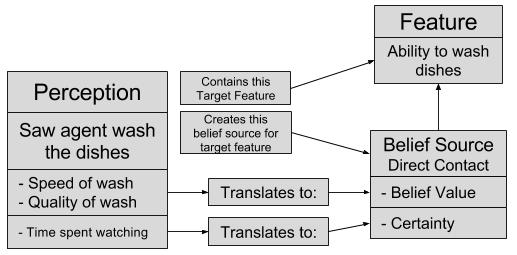
\includegraphics[width=200px]{PerceptionsDiagram.jpg}
    \caption{Perception Example}
    \label{fig:Perceptions Diagram}
\end{figure}

\subsection{Action Suggestion}
This component is meant to 
% A perception is mapped to relevant actions, and actions are allocated depending on time available and what is the lowest scoring relevant feature.

